% Options for packages loaded elsewhere
\PassOptionsToPackage{unicode}{hyperref}
\PassOptionsToPackage{hyphens}{url}
%
\documentclass[
  ignorenonframetext,
]{beamer}
\usepackage{pgfpages}
\setbeamertemplate{caption}[numbered]
\setbeamertemplate{caption label separator}{: }
\setbeamercolor{caption name}{fg=normal text.fg}
\beamertemplatenavigationsymbolsempty
% Prevent slide breaks in the middle of a paragraph
\widowpenalties 1 10000
\raggedbottom
\setbeamertemplate{part page}{
  \centering
  \begin{beamercolorbox}[sep=16pt,center]{part title}
    \usebeamerfont{part title}\insertpart\par
  \end{beamercolorbox}
}
\setbeamertemplate{section page}{
  \centering
  \begin{beamercolorbox}[sep=12pt,center]{part title}
    \usebeamerfont{section title}\insertsection\par
  \end{beamercolorbox}
}
\setbeamertemplate{subsection page}{
  \centering
  \begin{beamercolorbox}[sep=8pt,center]{part title}
    \usebeamerfont{subsection title}\insertsubsection\par
  \end{beamercolorbox}
}
\AtBeginPart{
  \frame{\partpage}
}
\AtBeginSection{
  \ifbibliography
  \else
    \frame{\sectionpage}
  \fi
}
\AtBeginSubsection{
  \frame{\subsectionpage}
}

\usepackage{amsmath,amssymb}
\usepackage{lmodern}
\usepackage{iftex}
\ifPDFTeX
  \usepackage[T1]{fontenc}
  \usepackage[utf8]{inputenc}
  \usepackage{textcomp} % provide euro and other symbols
\else % if luatex or xetex
  \usepackage{unicode-math}
  \defaultfontfeatures{Scale=MatchLowercase}
  \defaultfontfeatures[\rmfamily]{Ligatures=TeX,Scale=1}
\fi
\usetheme[]{theme/q-theme.scss}
% Use upquote if available, for straight quotes in verbatim environments
\IfFileExists{upquote.sty}{\usepackage{upquote}}{}
\IfFileExists{microtype.sty}{% use microtype if available
  \usepackage[]{microtype}
  \UseMicrotypeSet[protrusion]{basicmath} % disable protrusion for tt fonts
}{}
\makeatletter
\@ifundefined{KOMAClassName}{% if non-KOMA class
  \IfFileExists{parskip.sty}{%
    \usepackage{parskip}
  }{% else
    \setlength{\parindent}{0pt}
    \setlength{\parskip}{6pt plus 2pt minus 1pt}}
}{% if KOMA class
  \KOMAoptions{parskip=half}}
\makeatother
\usepackage{xcolor}
\newif\ifbibliography
\setlength{\emergencystretch}{3em} % prevent overfull lines
\setcounter{secnumdepth}{-\maxdimen} % remove section numbering


\providecommand{\tightlist}{%
  \setlength{\itemsep}{0pt}\setlength{\parskip}{0pt}}\usepackage{longtable,booktabs,array}
\usepackage{calc} % for calculating minipage widths
\usepackage{caption}
% Make caption package work with longtable
\makeatletter
\def\fnum@table{\tablename~\thetable}
\makeatother
\usepackage{graphicx}
\makeatletter
\def\maxwidth{\ifdim\Gin@nat@width>\linewidth\linewidth\else\Gin@nat@width\fi}
\def\maxheight{\ifdim\Gin@nat@height>\textheight\textheight\else\Gin@nat@height\fi}
\makeatother
% Scale images if necessary, so that they will not overflow the page
% margins by default, and it is still possible to overwrite the defaults
% using explicit options in \includegraphics[width, height, ...]{}
\setkeys{Gin}{width=\maxwidth,height=\maxheight,keepaspectratio}
% Set default figure placement to htbp
\makeatletter
\def\fps@figure{htbp}
\makeatother
\newlength{\cslhangindent}
\setlength{\cslhangindent}{1.5em}
\newlength{\csllabelwidth}
\setlength{\csllabelwidth}{3em}
\newlength{\cslentryspacingunit} % times entry-spacing
\setlength{\cslentryspacingunit}{\parskip}
\newenvironment{CSLReferences}[2] % #1 hanging-ident, #2 entry spacing
 {% don't indent paragraphs
  \setlength{\parindent}{0pt}
  % turn on hanging indent if param 1 is 1
  \ifodd #1
  \let\oldpar\par
  \def\par{\hangindent=\cslhangindent\oldpar}
  \fi
  % set entry spacing
  \setlength{\parskip}{#2\cslentryspacingunit}
 }%
 {}
\usepackage{calc}
\newcommand{\CSLBlock}[1]{#1\hfill\break}
\newcommand{\CSLLeftMargin}[1]{\parbox[t]{\csllabelwidth}{#1}}
\newcommand{\CSLRightInline}[1]{\parbox[t]{\linewidth - \csllabelwidth}{#1}\break}
\newcommand{\CSLIndent}[1]{\hspace{\cslhangindent}#1}

\makeatletter
\makeatother
\makeatletter
\makeatother
\makeatletter
\@ifpackageloaded{caption}{}{\usepackage{caption}}
\AtBeginDocument{%
\ifdefined\contentsname
  \renewcommand*\contentsname{Table of contents}
\else
  \newcommand\contentsname{Table of contents}
\fi
\ifdefined\listfigurename
  \renewcommand*\listfigurename{List of Figures}
\else
  \newcommand\listfigurename{List of Figures}
\fi
\ifdefined\listtablename
  \renewcommand*\listtablename{List of Tables}
\else
  \newcommand\listtablename{List of Tables}
\fi
\ifdefined\figurename
  \renewcommand*\figurename{Figure}
\else
  \newcommand\figurename{Figure}
\fi
\ifdefined\tablename
  \renewcommand*\tablename{Table}
\else
  \newcommand\tablename{Table}
\fi
}
\@ifpackageloaded{float}{}{\usepackage{float}}
\floatstyle{ruled}
\@ifundefined{c@chapter}{\newfloat{codelisting}{h}{lop}}{\newfloat{codelisting}{h}{lop}[chapter]}
\floatname{codelisting}{Listing}
\newcommand*\listoflistings{\listof{codelisting}{List of Listings}}
\makeatother
\makeatletter
\@ifpackageloaded{caption}{}{\usepackage{caption}}
\@ifpackageloaded{subcaption}{}{\usepackage{subcaption}}
\makeatother
\makeatletter
\@ifpackageloaded{tcolorbox}{}{\usepackage[many]{tcolorbox}}
\makeatother
\makeatletter
\@ifundefined{shadecolor}{\definecolor{shadecolor}{rgb}{.97, .97, .97}}
\makeatother
\makeatletter
\makeatother
\ifLuaTeX
  \usepackage{selnolig}  % disable illegal ligatures
\fi
\IfFileExists{bookmark.sty}{\usepackage{bookmark}}{\usepackage{hyperref}}
\IfFileExists{xurl.sty}{\usepackage{xurl}}{} % add URL line breaks if available
\urlstyle{same} % disable monospaced font for URLs
\hypersetup{
  hidelinks,
  pdfcreator={LaTeX via pandoc}}

\author{}
\date{}
\logo{\includegraphics{img/HYU\_logo\_singlecolor\_png.png}}

\begin{document}
\ifdefined\Shaded\renewenvironment{Shaded}{\begin{tcolorbox}[borderline west={3pt}{0pt}{shadecolor}, enhanced, sharp corners, interior hidden, frame hidden, boxrule=0pt, breakable]}{\end{tcolorbox}}\fi

\begin{frame}[fragile]
OTT Movie Launching Strategy

with Movie-Country Relatedness

2023 한국언론학회 봄철 정기학술대회\\
\texttt{미디어\ 경제/경영\ 연구회}

2023-05-19

Changjun Lee

Hanyang University

Dep. Media \& Social Informatics


\includegraphics[width=1.12em,height=1em]{index_files/figure-beamer/fa-icon-9de8c0f3cb50e30659d3ab543abf8bca.pdf}
~\href{https://changjunlee.com/}{changjunlee.com}
\end{frame}

\begin{frame}[fragile]{We are..}
\protect\hypertarget{we-are..}{}
\begin{block}{일반공동연구지원사업(인문사회)}
\protect\hypertarget{uxc77cuxbc18uxacf5uxb3d9uxc5f0uxad6cuxc9c0uxc6d0uxc0acuxc5c5uxc778uxbb38uxc0acuxd68c}{}
\begin{block}{한국연구재단(2020S1A5A2A0304148012)}
\protect\hypertarget{uxd55cuxad6duxc5f0uxad6cuxc7acuxb2e82020s1a5a2a0304148012}{}
\begin{columns}[T]
\begin{column}{0.23\textwidth}
\end{column}

\begin{column}{0.18\textwidth}
\textbf{연구 책임자}

\includegraphics[width=3.125in,height=\textheight]{img/ji.gif}

\begin{block}{지성욱 교수}
\protect\hypertarget{uxc9c0uxc131uxc6b1-uxad50uxc218}{}
\end{block}

\begin{block}{\texttt{한국외대}}
\protect\hypertarget{uxd55cuxad6duxc678uxb300}{}
\end{block}
\end{column}

\begin{column}{0.18\textwidth}
\textbf{공동 연구자}


\includegraphics[width=3.125in,height=\textheight]{img/lsy.jpg}

\begin{block}{이상엽 교수}
\protect\hypertarget{uxc774uxc0c1uxc5fd-uxad50uxc218}{}
\end{block}

\begin{block}{\texttt{연세대}}
\protect\hypertarget{uxc5f0uxc138uxb300}{}
\end{block}
\end{column}

\begin{column}{0.18\textwidth}
\textbf{공동 연구자}


\includegraphics[width=3.125in,height=\textheight]{img/cj.jpg}

\begin{block}{이창준 교수}
\protect\hypertarget{uxc774uxcc3duxc900-uxad50uxc218}{}
\end{block}

\begin{block}{\texttt{한양대ERICA}}
\protect\hypertarget{uxd55cuxc591uxb300erica}{}
\end{block}
\end{column}

\begin{column}{0.23\textwidth}
\end{column}
\end{columns}
\end{block}
\end{block}
\end{frame}

\begin{frame}[fragile]{Research Background}
\protect\hypertarget{research-background}{}
\begin{block}{Global OTT Platforms and Cultural Barriers}
\protect\hypertarget{global-ott-platforms-and-cultural-barriers}{}
\begin{itemize}
\item
  Emergence of global OTTs: \texttt{Netflix}, \texttt{Disney+}, etc.
\item
  Lowering cultural barriers in media consumption
\item
  Examples:

  \begin{itemize}
  \item
    Korean TV shows: \texttt{Squid\ Game},
    \texttt{Extraordinary\ Attorney\ Woo} (CNN 2022)
  \item
    US-based show: \texttt{Strange\ Things} (Reporter 2022)
  \end{itemize}
\item
  However, \textbf{Global mega-hits still rare}, often a matter of
  serendipity
\end{itemize}

\begin{columns}[T]
\begin{column}{0.5\textwidth}

\includegraphics[width=8.33333in,height=\textheight]{img/ott_3.jpg}
\end{column}

\begin{column}{0.25\textwidth}

\includegraphics[width=\textwidth,height=4.6875in]{img/ott_1.jpg}
\end{column}

\begin{column}{0.25\textwidth}

\includegraphics[width=\textwidth,height=4.6875in]{img/ott_2.jpg}
\end{column}
\end{columns}
\end{block}
\end{frame}

\begin{frame}[fragile]{Research Background}
\protect\hypertarget{research-background-1}{}
\begin{block}{\textbf{Local Media Channels and OTTs -
\texttt{Challenges}}}
\protect\hypertarget{local-media-channels-and-otts---challenges}{}
\begin{itemize}
\item
  Global OTTs threaten local media channels
\item
  Local OTTs emerge to counter competition
\item
  Main challenges for local OTTs:

  \begin{enumerate}
  \item
    Producing culturally appropriate content with global mega-hit
    potential
  \item
    Renting overseas content that appeals to local users (Wang and Jung
    2023)
  \end{enumerate}
\end{itemize}

\begin{columns}[T]
\begin{column}{0.3\textwidth}
\end{column}

\begin{column}{0.5\textwidth}
\begin{figure}

\includegraphics[width=9.375in,height=\textheight]{https://assets.mspimages.in/gear/wp-content/uploads/2022/11/tv-6860973_960_720.jpg} \hfill{}

\end{figure}
\end{column}
\end{columns}

Source: mysmartprice (Abhijith 2022)
\end{block}
\end{frame}

\begin{frame}{Research Background}
\protect\hypertarget{research-background-2}{}
\begin{block}{\textbf{Strategies for Local OTT Success}}
\protect\hypertarget{strategies-for-local-ott-success}{}
\begin{itemize}
\item
  Addressing purchasing priority and cost-effectiveness
\item
  Creating high-quality content with worldwide resonance (Kim 2022)
\item
  Catering to local user preferences
\item
  Latecomer local OTT operators need additional strategies
\end{itemize}

\begin{figure}

{\centering 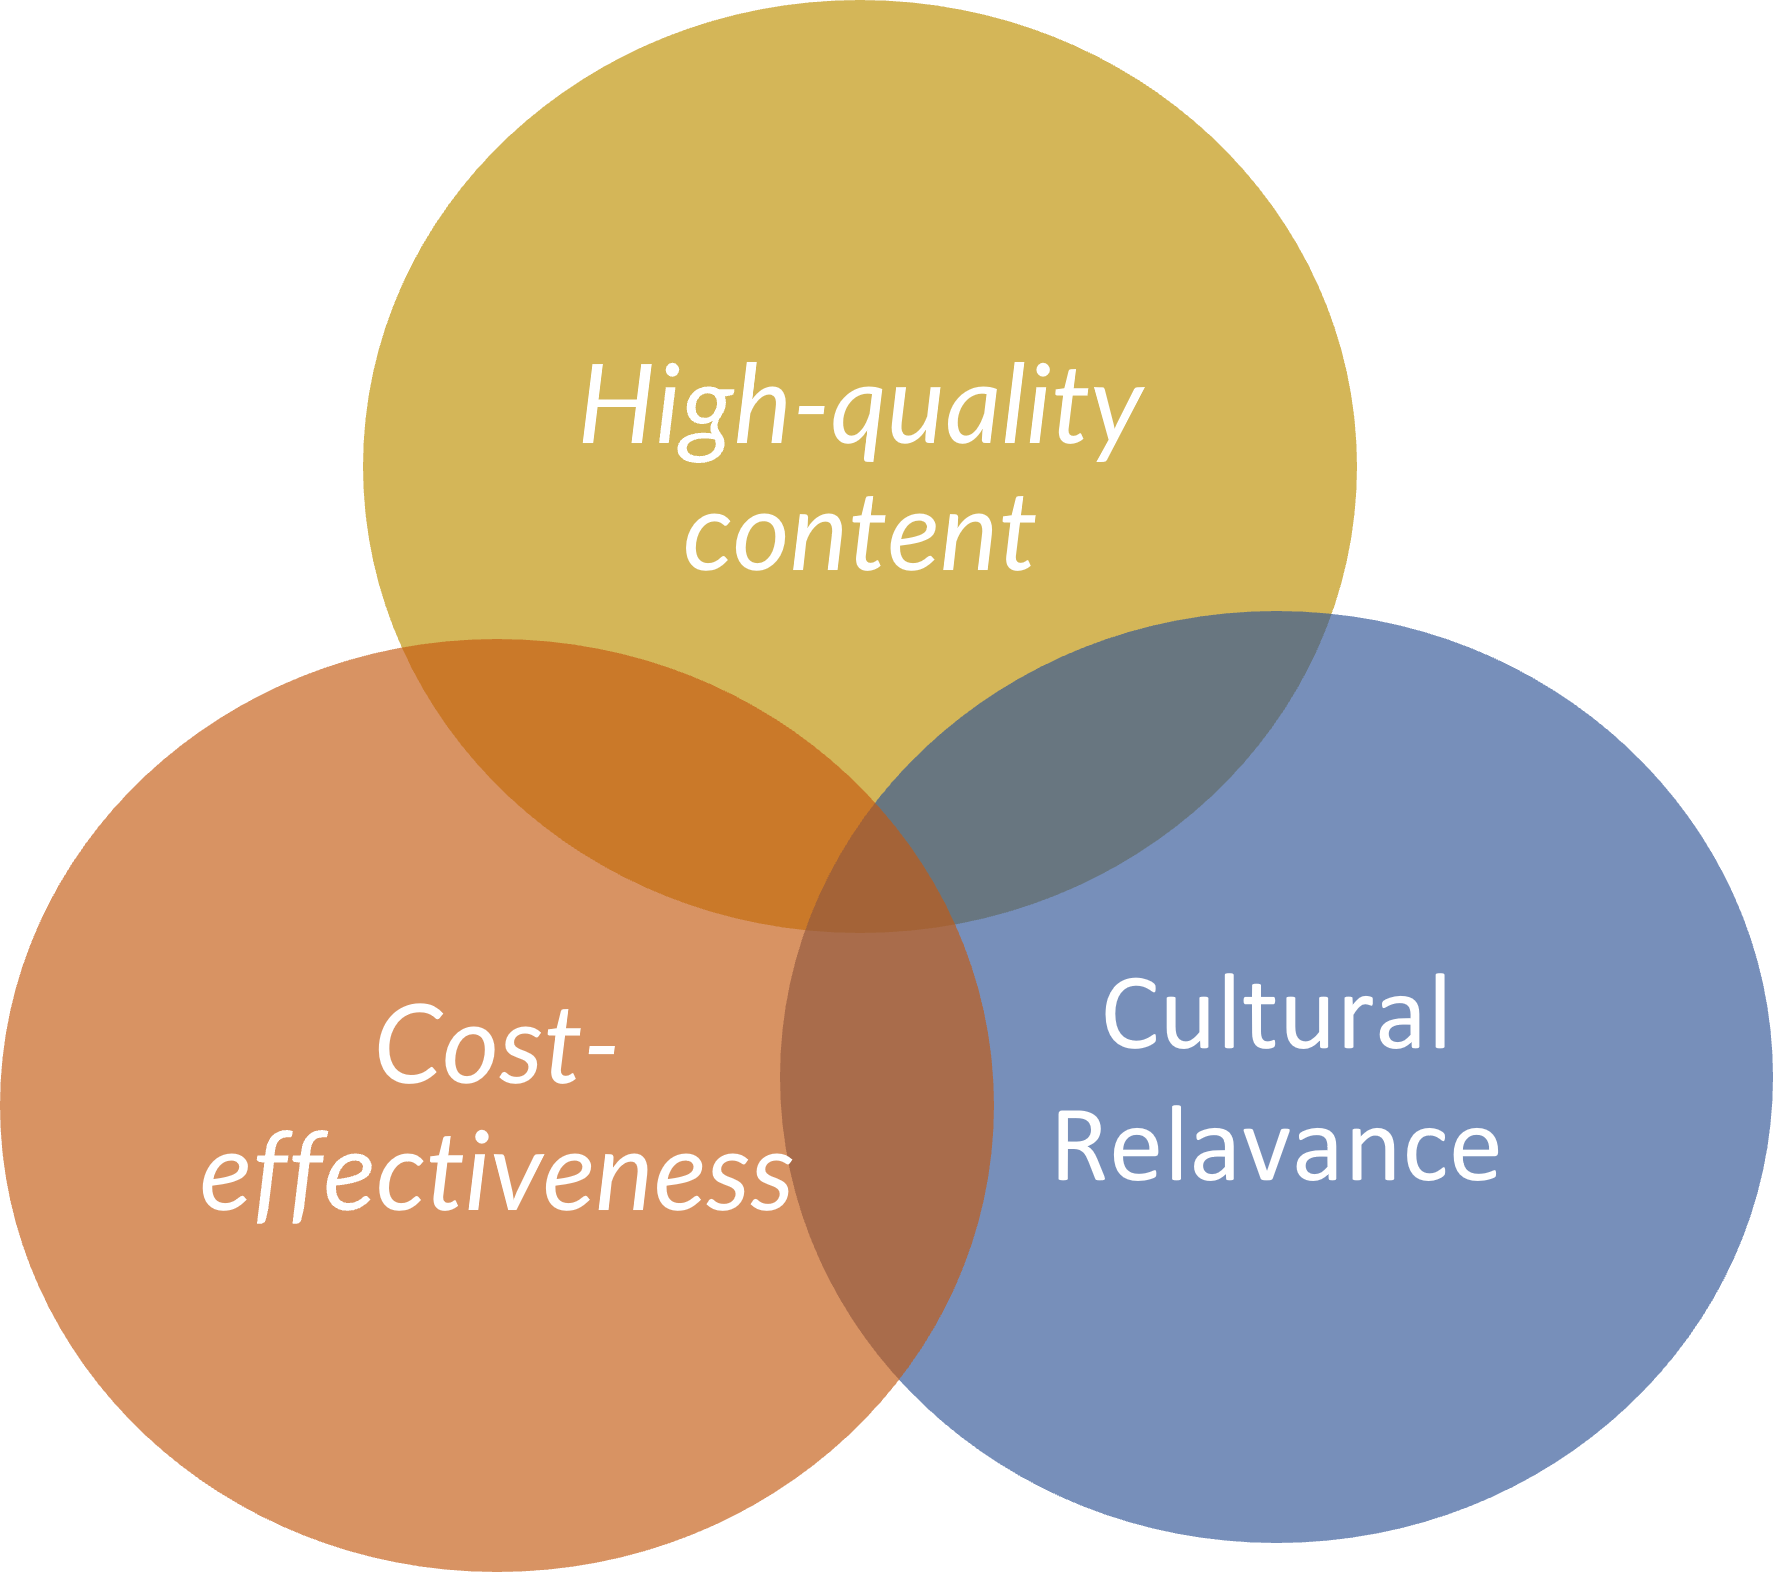
\includegraphics{img/fig_3.png}

}

\end{figure}
\end{block}
\end{frame}

\begin{frame}[fragile]{Problem Description}
\protect\hypertarget{problem-description}{}
\begin{itemize}
\item
  Previous research on OTT strategies (Park and Kwon 2019)

  \begin{itemize}
  \tightlist
  \item
    Localization, Partnership, Content differentiation, Revenue
    enhancement, Service optimization
  \end{itemize}
\item
  Local OTT providers adopt a multi-faceted approach

  \begin{itemize}
  \item
    Assessing demand and establishing partnerships (Wang and Jung 2023)

    \begin{itemize}
    \tightlist
    \item
      Acquiring content similar in genre and quality to Netflix and
      Disney+
    \end{itemize}
  \item
    Developing local content repositories using local/regional languages
    (Sharma and Lulandala 2023)

    \begin{itemize}
    \tightlist
    \item
      Forming strategic collaborations with: Mobile network companies,
      Financial institutions, Technology companies
    \end{itemize}
  \end{itemize}
\end{itemize}

\textbf{Research Gap}

\begin{itemize}
\item
  Limited understanding of OTT launching strategies considering:

  \begin{itemize}
  \tightlist
  \item
    \texttt{Compatibility} between movies and countries
  \end{itemize}
\item
  Need for more research on country-specific content and strategies
\end{itemize}
\end{frame}

\begin{frame}{Research Questions \& Goal}
\protect\hypertarget{research-questions-goal}{}
\textbf{Research Questions}

\begin{itemize}
\item
  How do content and country relationships impact popularity?
\item
  How can accurate measurements of relatedness improve content
  consumption patterns?
\end{itemize}

\textbf{Research Goal}

\begin{itemize}
\item
  Propose a method to measure \textbf{\emph{movie-country relatedness
  density}}
\item
  Test the importance of the \textbf{\emph{movie-country relatedness}}
  in predicting \textbf{\emph{movie popularity}} in specific countries
\item
  Develop \textbf{\emph{a local OTT strategy}} based on movie-country
  relatedness
\end{itemize}
\end{frame}

\begin{frame}{Theoretical Foundations}
\protect\hypertarget{theoretical-foundations}{}
\textbf{The Complexity of the Cultural Industry}

\begin{itemize}
\item
  Cultural goods difficult to express as utility function (Throsby 2001)
\item
  Cultural industry sectors:

  \begin{itemize}
  \item
    Media
  \item
    Fashionable consumer goods
  \item
    Services
  \item
    Creative professions
  \item
    Collective cultural consumption institutions (Scott 2004)
  \end{itemize}
\end{itemize}

\emph{Recommended picture: A collage of various cultural industry
elements (e.g., film, music, architecture, art).}
\end{frame}

\begin{frame}{Theoretical Foundations}
\protect\hypertarget{theoretical-foundations-1}{}
\textbf{Cultural Sensitivity in International Trade}

\begin{itemize}
\item
  Content carries cultural messages (Fejes 1981)
\item
  Protection of local content from other markets
\item
  Cultural goods deeply rooted in their place of origin (Demont‐Heinrich

  \begin{enumerate}
  [1)]
  \setcounter{enumi}{2010}
  \tightlist
  \item
  \end{enumerate}
\item
  Globalization and multicultural companies impact the cultural economy
\end{itemize}

\emph{Recommended picture: A map with arrows showing the flow of
cultural goods between countries, indicating the sensitivity of
international trade in cultural goods.}
\end{frame}

\begin{frame}{Theoretical Foundations}
\protect\hypertarget{theoretical-foundations-2}{}
\textbf{Cultural Similarity and Content-Country Compatibility}

\begin{itemize}
\item
  Importance of cultural similarity in adopting foreign content (Dwyer
  et al.~2018, Jang et al.~2023, Kim 2022, Sharma and Lulandala 2023)
\item
  Shared cultural attributes due to content globalization
\item
  Special content--country compatibility beyond cultural differences
\item
  Borrowing the concept of product--country compatibility from economic
  geography (Hausmann and Hidalgo 2010)
\end{itemize}

\emph{Recommended picture: A Venn diagram showing the overlap of
cultural similarity and content-country compatibility.}
\end{frame}

\begin{frame}{Theoretical Foundations}
\protect\hypertarget{theoretical-foundations-3}{}
\textbf{Product-Country Compatibility}

\begin{itemize}
\item
  Concept from economic geography
\item
  Considers cultural, economic, and regulatory conditions (Asheim and
  Isaksen 2002)
\item
  Impacts a product's success in a target market
\item
  Compatibility evaluated through relatedness (Jun et al.~2020)

  \begin{enumerate}
  \item
    Product relatedness
  \item
    Importer relatedness
  \item
    Exporter relatedness
  \end{enumerate}
\end{itemize}

\emph{Recommended picture: A diagram illustrating the three dimensions
of relatedness (product, importer, and exporter).}
\end{frame}

\begin{frame}{Theoretical Foundations}
\protect\hypertarget{theoretical-foundations-4}{}
\textbf{The Importance of Product-Country Compatibility}

\begin{itemize}
\item
  Widely recognized in international business and economic geography
  (Cavusgil et al.~2014)
\item
  Culturally aligned products more likely to succeed
\item
  Compatibility with economic and regulatory environment leads to
  profitability
\end{itemize}

\emph{Recommended picture: A graph showing the relationship between
product-country compatibility and product success in a foreign market.}
\end{frame}

\begin{frame}{Theoretical Foundations}
\protect\hypertarget{theoretical-foundations-5}{}
\textbf{Applying Product-Country Compatibility to Content}

\begin{itemize}
\item
  Adapting the concept for content-country compatibility
\item
  Assessing cultural, economic, and regulatory fit for content in target
  countries
\item
  Potential to improve the success of content in foreign markets
\end{itemize}

\emph{Recommended picture: A split image, with one side showing a
product and its compatibility with a country, and the other side showing
content and its compatibility with a country, illustrating the
connection between the two concepts.}
\end{frame}

\begin{frame}{Theoretical Foundations}
\protect\hypertarget{theoretical-foundations-6}{}
\textbf{Content-Country Compatibility}

\begin{itemize}
\item
  Adaptation of product-country compatibility for movies and TV shows
\item
  Considers cultural, economic, and regulatory conditions
\item
  Impacts success and profitability of content in target markets
\end{itemize}

\emph{Recommended picture: A diagram illustrating the factors that
contribute to content-country compatibility (cultural, economic, and
regulatory conditions).}
\end{frame}

\begin{frame}{Theoretical Foundations}
\protect\hypertarget{theoretical-foundations-7}{}
\textbf{Importance of Content-Country Compatibility}

\begin{itemize}
\item
  Aligns with research on product-country compatibility
\item
  Successful content aligns with a country's cultural norms, values, and
  legal framework
\item
  Examples: local actors, settings, themes
\end{itemize}

\emph{Recommended picture: A collage of successful movies and TV shows
in various countries, illustrating the importance of content-country
compatibility.}
\end{frame}

\begin{frame}{Theoretical Foundations}
\protect\hypertarget{theoretical-foundations-8}{}
\textbf{Factors Influencing Content-Country Compatibility}

\begin{itemize}
\item
  Cultural factors: language, humor, storytelling style
\item
  Economic factors: disposable income, streaming service accessibility
\item
  Regulatory factors: censorship laws, import/export regulations
\item
  Complex interplay of factors in evaluating potential success
\end{itemize}

\emph{Recommended picture: A Venn diagram showing the overlap of
cultural, economic, and regulatory factors influencing content-country
compatibility.}
\end{frame}

\begin{frame}{Theoretical Foundations}
\protect\hypertarget{theoretical-foundations-9}{}
\textbf{Summary}

\begin{itemize}
\item
  Content-country compatibility crucial for international expansion
\item
  Align content with target country's cultural, economic, and regulatory
  conditions
\item
  Increases likelihood of success in international business endeavors
\end{itemize}

\emph{Recommended picture: A globe with arrows pointing to various
countries, symbolizing the international expansion of content and the
importance of content-country compatibility.}
\end{frame}

\begin{frame}{Theoretical Foundations}
\protect\hypertarget{theoretical-foundations-10}{}
\textbf{Measuring Content-Movie Compatibility}

\begin{itemize}
\item
  Use relatedness density index to measure content-movie compatibility
\item
  Equation (1) for calculating content-country related density
  (〖RD〗\_(r,i))
\item
  Considers co-occurrence of top-tiered lists to measure relatedness
  (∅\_(i,j))
\end{itemize}

\emph{Recommended picture: A diagram illustrating the calculation of
content-country related density using the relatedness density index.}
\end{frame}

\begin{frame}{Theoretical Foundations}
\protect\hypertarget{theoretical-foundations-11}{}
\textbf{Variation in Movies and TV Shows}

\begin{itemize}
\item
  Movies and TV shows vary in themes, characters, cultural references
\item
  Impacts compatibility with specific countries due to diverse cultural
  norms, values, preferences
\end{itemize}

\emph{Recommended picture: A collage of movies and TV shows with varying
themes, characters, and cultural references to illustrate the diversity
in content.}
\end{frame}

\begin{frame}{Hypothesis}
\protect\hypertarget{hypothesis}{}
\textbf{Hypothesis 1}

\begin{itemize}
\item
  H1: Movies and TV shows exhibit varying degrees of compatibility with
  different countries
\item
  Compatibility predicts a given country's likelihood of including
  content in its top 20 list
\end{itemize}

\emph{Recommended picture: A bar chart showing varying degrees of
compatibility for different movies and TV shows across different
countries, illustrating the hypothesis.}
\end{frame}

\begin{frame}{Hypothesis}
\protect\hypertarget{hypothesis-1}{}
\textbf{Hypothesis 2}

\begin{itemize}
\item
  Importance of content-country compatibility acknowledged
\item
  Global mega-hit content occasionally becomes popular across various
  countries, regardless of compatibility
\item
  Factors contributing to widespread popularity: effective marketing,
  favorable media coverage, word-of-mouth recommendations
\item
  Hypothesis 2: Ubiquity of popular content predicts a given country's
  likelihood of including that content in its top 20 list
\end{itemize}

\emph{Recommended picture: A world map showing the widespread popularity
of a global mega-hit movie or TV show, illustrating the hypothesis.}
\end{frame}

\begin{frame}{Methods}
\protect\hypertarget{methods}{}
\textbf{Method Overview}

\begin{itemize}
\item
  Data source: Flixpatrol's monthly top 20 movies in 80 countries from
  January to December 2021
\item
  Final sample: 1,939 movies (1,861,440 observations)
\item
  Focusing on Netflix as a global OTT service provider
\item
  Dependent variable: 〖ENT\_TOP20〗\_(c,m,t+1) - new entry of a movie m
  in a country's top 20 list in the period t+1
\end{itemize}

\emph{Recommended picture: A world map showing the countries included in
the study, with each country having a top 20 list icon.}
\end{frame}

\begin{frame}{Methods}
\protect\hypertarget{methods-1}{}
\textbf{Independent Variables and Covariates}

\begin{itemize}
\item
  Independent variables:

  \begin{itemize}
  \item
    Country--movie relatedness density (∅\_(c,m,t))
  \item
    Movie ubiquity (U\_(m,t))
  \end{itemize}
\item
  Covariates:

  \begin{itemize}
  \tightlist
  \item
    Movie-specific fixed effects (Z\_(m,t)): Netflix Original status,
    production country, genre, Rotten Tomatoes score, and IMDB score
  \end{itemize}
\item
  Purpose: Account for factors influencing a movie's inclusion in a
  country's top 20 list
\end{itemize}

\emph{Recommended picture: A chart or diagram illustrating the
relationships between the dependent variable, independent variables, and
covariates in the model.}
\end{frame}

\begin{frame}{Methods}
\protect\hypertarget{methods-2}{}
\textbf{Descriptive Statistics}

\begin{itemize}
\item
  Variables in the study:

  \begin{itemize}
  \item
    TOP20 Dummy: binary, 1.0\% of observations = 1
  \item
    Entry Dummy: binary, 0.9\% of observations = 1
  \item
    Netflix Original: binary, 12.8\% of movies = Netflix Originals
  \item
    Related Density: mean = 0.2, standard deviation = 0.2, range = 0 to
    1
  \item
    Movie Ubiquity: mean = 0.0, standard deviation = 0.1, range = 0 to
    80
  \item
    IMDB Score: mean = 6.3, standard deviation = 1.1
  \item
    Rotten Tomatoes Score: mean = 53.6, standard deviation = 25.9
  \item
    Genre: Action, Comedy, Drama, Science Fiction, and Etc.
  \item
    Producing Country: country where a movie was produced
  \item
    Month in 2021: each month has 9.1\% of the total sample
  \end{itemize}
\end{itemize}

\emph{Recommended picture: A table or chart showing the descriptive
statistics for each variable.}
\end{frame}

\begin{frame}{Methods}
\protect\hypertarget{methods-3}{}
\textbf{Descriptive Statistics by Entry Status}

\begin{itemize}
\item
  1,706,320 observations, 15,561 (0.9\%) movies newly entered top 20
\item
  Statistically significant differences (p \textless{} .001):

  \begin{itemize}
  \item
    Related Density: Entry = 1 (0.5 ± 0.2), Entry = 0 (0.2 ± 0.2)
  \item
    Movie Ubiquity: Entry = 1 (0.4 ± 0.4), Entry = 0 (0.0 ± 0.0)
  \item
    Netflix Original: Entry = 1 (44.8\%), Entry = 0 (12.8\%)
  \item
    Genre and Producing Country proportions
  \end{itemize}
\item
  No statistically significant differences:

  \begin{itemize}
  \item
    IMDB Score: Entry = 1 (6.3 ± 1.0), Entry = 0 (6.4 ± 1.1)
  \item
    Rotten Tomatoes Score
  \end{itemize}
\end{itemize}

\emph{Recommended picture: A table or chart showing the descriptive
statistics for each variable by entry status.}
\end{frame}

\begin{frame}{Results}
\protect\hypertarget{results}{}
\textbf{Results Overview}

\begin{itemize}
\item
  Three models analyzing relationship between dependent variable
  (〖ENT\_TOP20〗\_(c,m,t+1)) and independent variables
\item
  Model 1: Related Density and Movie Ubiquity only
\item
  Model 2 \& Model 3: Additional variables (IMDB Score, Rotten Tomatoes
  Score, Netflix Original, Genre, Producing Country, Monthly Fixed
  Effects)
\end{itemize}

\emph{Recommended picture: A table showing the results of the three
models for each variable.}
\end{frame}

\begin{frame}{Results}
\protect\hypertarget{results-1}{}
\textbf{Key Findings}

\begin{itemize}
\item
  Related Density and Movie Ubiquity positively associated with
  dependent variable in all models

  \begin{itemize}
  \tightlist
  \item
    Suggests relatedness to other popular movies and worldwide
    popularity important for top 20 appearance
  \end{itemize}
\item
  Other significant predictors in Model 2 \& Model 3:

  \begin{itemize}
  \item
    Positive: Higher IMDB score
  \item
    Negative: Higher Rotten Tomatoes score
  \item
    Netflix Original: Positive in Model 1, Negative in Model 3
  \item
    Genre and Producing Country: Significant variation in coefficients
  \end{itemize}
\end{itemize}

\emph{Recommended picture: A chart or graph visualizing the significant
predictors and their associations with the dependent variable.}
\end{frame}

\begin{frame}{Discussion}
\protect\hypertarget{discussion}{}
\textbf{Conclusions}

\begin{itemize}
\item
  Relatedness and ubiquity are important factors in predicting top 20
  appearance
\item
  Other factors also play a significant role in predicting likelihood of
  appearing in a country's top 20 list
\end{itemize}

\emph{Recommended picture: A visual summary of the key findings and
their implications for understanding movie popularity.}
\end{frame}

\begin{frame}{Discussion}
\protect\hypertarget{discussion-1}{}
\textbf{Main Findings and Implications}

\begin{itemize}
\item
  Related Density and Movie Ubiquity positively associated with top 20
  list appearance
\item
  Hypotheses supported: Content-country compatibility and global
  popularity impact top 20 list inclusion
\item
  Other significant predictors: IMDB Score, Rotten Tomatoes Score,
  Netflix Original, Genre, Producing Country, Monthly F.E.
\item
  Findings suggest importance of considering country--movie related
  density for OTT movie launching strategy
\end{itemize}

\emph{Recommended picture: A chart or graph summarizing the main
findings and their implications for understanding movie popularity.}
\end{frame}

\begin{frame}{Discussion}
\protect\hypertarget{discussion-2}{}
\textbf{OTT Content Launching Strategy Map}

\begin{itemize}
\item
  X-axis: Country--movie related density
\item
  Y-axis: Movie ubiquity
\item
  Quadrant 1 (High related density, high ubiquity): Low-risk,
  high-benefit section

  \begin{itemize}
  \tightlist
  \item
    High investment, high return potential due to global popularity
  \end{itemize}
\item
  Suggested strategy: Local OTT providers focus on movies in Quadrant 1
\end{itemize}

\emph{Recommended picture: A visual representation of the OTT content
launching strategy map, with quadrants highlighting the different
combinations of related density and movie ubiquity.}
\end{frame}

\begin{frame}{Discussion}
\protect\hypertarget{discussion-3}{}
\textbf{Quadrants of OTT Content Launching Strategy}

\begin{itemize}
\item
  Quadrant 2: High ubiquity, low related density

  \begin{itemize}
  \tightlist
  \item
    Moderate-risk option due to limited local appeal
  \end{itemize}
\item
  Quadrant 4: Low ubiquity, high related density

  \begin{itemize}
  \tightlist
  \item
    Low-cost, low-profit, but potential for unexpected profits due to
    local user compatibility
  \end{itemize}
\end{itemize}

\emph{Recommended picture: A chart or graph illustrating the quadrants
of the OTT content launching strategy map.}
\end{frame}

\begin{frame}{Discussion}
\protect\hypertarget{discussion-4}{}
\textbf{Country-Specific OTT Content Launching Maps}

\begin{itemize}
\item
  Argentina (December 2021):

  \begin{itemize}
  \item
    Red dots: Top 20 content
  \item
    Black dots: Not yet in top 20
  \item
    Examples of famous movies with low compatibility: A Castle for
    Christmas, A Boy Called Christmas, Single All the Way
  \item
    Examples of locally compatible, less known movies: I Feel Pretty,
    Waiting for the Hearse
  \end{itemize}
\item
  United States (December 2021):

  \begin{itemize}
  \item
    Examples of famous movies with low compatibility: Spiderman
    Homecoming, Spoiled Brats, Anonymously Yours
  \item
    Examples of locally compatible, less known movies: Love Happens, 21
    Jump Street, American Me
  \end{itemize}
\item
  South Korea: Refer to Figure 7
\end{itemize}

\textbf{Contribution to Research}

\begin{itemize}
\item
  Adds to the growing body of research on movie consumption patterns
\item
  Provides insights into factors determining movie success globally
\item
  Helps local OTT providers tailor content to local audiences and
  compete with global players
\end{itemize}
\end{frame}

\begin{frame}{Future Plans}
\protect\hypertarget{future-plans}{}
\begin{itemize}
\tightlist
\item
  Robustness check
\end{itemize}

\begin{itemize}
\item
  Explore more..

  \begin{itemize}
  \item
    e.g.) Multi-perosonal tendency clustering
  \item
    Explore any difference in metaverse usage among clusters
  \end{itemize}
\end{itemize}

\begin{itemize}
\tightlist
\item
  Wrapping up the results and find a target journal
\end{itemize}
\end{frame}

\begin{frame}{Finalize this talk}
\protect\hypertarget{finalize-this-talk}{}
\begin{block}{Thanks for your attention}
\protect\hypertarget{thanks-for-your-attention}{}
You can find this presentation here

\begin{itemize}
\tightlist
\item
  \url{https://changjunlee.com/blogs/posts/7_avatar_custo.html}
\end{itemize}
\end{block}

\begin{block}{Any questions \& suggestions?}
\protect\hypertarget{any-questions-suggestions}{}
Changjun Lee

Hanyang University

Dep. Media \& Social Informatics


\includegraphics[width=1.12em,height=1em]{index_files/figure-beamer/fa-icon-9de8c0f3cb50e30659d3ab543abf8bca.pdf}
~\href{https://changjunlee.com/}{changjunlee.com}


\includegraphics[width=5.20833in,height=\textheight]{img/my_avatar.png}
\end{block}
\end{frame}

\begin{frame}{References}
\protect\hypertarget{references}{}
\hypertarget{refs}{}
\begin{CSLReferences}{1}{0}
\leavevmode\vadjust pre{\hypertarget{ref-fig_ott_1}{}}%
Abhijith. 2022. {``OTT Full Form: Meaning, How Does It Work, Popular OTT
Platforms in India, Price, and More.''} \emph{Mysmartprice}, November.
\url{https://www.mysmartprice.com/gear/ott-full-form-meaning-popular-ott-platforms/}.

\leavevmode\vadjust pre{\hypertarget{ref-cnn2022attorneywoo}{}}%
CNN. 2022. {``{`Extraordinary Attorney Woo'} Boosts Netflix Stock.''}
\url{https://edition.cnn.com/2022/07/20/media/extraordinary-attorney-woo-netflix-stock-intl-hnk/index.html}.

\leavevmode\vadjust pre{\hypertarget{ref-kim2022theorizing}{}}%
Kim, T. 2022. {``Theorizing the Korean Wave\textbar{} k-Culture Without
{`k-'}? The Paradoxical Nature of Producing Korean Television Toward a
Sustainable Korean Wave.''} \emph{International Journal of
Communication} 17: 22.

\leavevmode\vadjust pre{\hypertarget{ref-park2019research}{}}%
Park, S., and Y. Kwon. 2019. {``Research on the Relationship Between the
Growth of OTT Service Market and the Change in the Structure of the
Pay-TV Market.''} \emph{Journal of Digital Convergence} 17: 15--28.

\leavevmode\vadjust pre{\hypertarget{ref-hollywoodreporter2022strangerthings}{}}%
Reporter, The Hollywood. 2022. {``{`Stranger Things 4'} Sets All-Time
Nielsen Streaming Record.''}
\url{https://www.hollywoodreporter.com/tv/tv-news/stranger-things-4-all-time-nielsen-streaming-high-1235174960/}.

\leavevmode\vadjust pre{\hypertarget{ref-sharma2023ott}{}}%
Sharma, K., and E. E. Lulandala. 2023. {``OTT Platforms Resilience to
COVID-19--a Study of Business Strategies and Consumer Media Consumption
in India.''} \emph{International Journal of Organizational Analysis} 31:
63--90.

\leavevmode\vadjust pre{\hypertarget{ref-wang2023influential}{}}%
Wang, S.-H., and Y. Jung. 2023. {``Influential Factors in Domestic OTT
Platforms' Choice of Foreign Content in South Korea.''}
\emph{International Journal on Media Management}, 1--27.

\end{CSLReferences}
\end{frame}



\end{document}
